\chapter{Transient Laser Behaviour}
\graphicspath{{./cap_6/images/}}

\section{Q-switching di un laser I: aspetti dinamici}
Un laser emette uno o una sequenza periodica di impulsi "giganti" di luce, della durata $\D\tau_p$ di pochi o decine di nanosecondi e potenze di picco $P_{peak} \sim 10 MW - 1 GW$.
%disegno
Rispetto ad un laser che opera in onda continua (CW), la potenza di picco è molto superiore (ad es. nei laser a $CO_2$ o laser a stato solido in fibra, $P_{out}$ raggiunge valori al massimo fino a $100-200 kW$). Il regime di Q-switching è possibile solo per laser con tempo $\tau$ del livello laser superiore lungo ($\tau$ da 10 $\mu$s a $ms$), come nei laser a stato solido.\\
\\
L'idea alla base del funzionamento in Q-switching di un laser è quello di commutare il fattore Q del risonatore da un valore basso (in cui il laser è sotto soglia ed il pompaggio consente di realizzare una elevata inversione di popolazione $N_i$) ad un valore alto in tempi brevi ($< \sim 100 ns$): in tale condizione, $N_i$ è molto maggiore di $N_{th}$ del laser (con Q alto) e l'elevata amplificazione nel mezzo attivo dei fotoni, a partire dell'extra fotone di emissione spontanea, converte l'energia interna immagazzinata nel mezzo attivo in un impulso "gigante", cioè molto energetico di breve $\D\tau_p \sim 1 ns - 10 ns$.\\
\\
Il Q-switching contrariamente al mode locking è sostanzialmente un regime di singolo modo e può quindi essere studiato utilizzando le rate-eq. del laser.
\begin{description}
\item [I fase] Q basso.
Il laser è sotto soglia (per cui $\phi \simeq 0$), per cui
\begin{equation*}
\dot{N} = R_p -\frac{N}{\tau}
\end{equation*}
Se $R_p$ è un "gradino" al tempo $t=0$, la soluzione dell'eq. differenziale di $N(t)$:
\begin{equation*}
N(t) = R_p\tau\left(1 - e^{-\frac{t}{\tau}}\right)
\end{equation*}
Dopo un tempo $t=t_s$ dell'ordine di $2-3 \tau$ tempo di switching, commuto da basso ad alto. L'inversione di popolazione accumulata nel mezzo attivo al tempo $t=t_s$ di switching vale $N(t) = R_p\tau\left(1 - e^{-\frac{t_s}{\tau}}\right) \approx R_p\tau$\\

Al fine di avere $N_i$ elevato senza pompare in maniera estrema, occorre che $\tau$ sia lungo quindi laser a stato solido (transizioni debolmente permesse per dipolo elettrico $\tau$ tra $\o \mu s - ms$).
\item [II fase] Q alto.
Devo distinguere due casi:
\begin{enumerate}
\item fast switching dove cioè $\gamma(t)$ varia dal valore alto al basso "istantaneamente". Per copiare le funzioni dell'impulso di Q-switching, devo studiare (ad es. numericamente) la dinamica delle rate-eq.
\begin{equation*}
\begin{cases}
\dot{N} = R_p - \frac{N}{\tau} - B\phi N\\
\dot{\phi} = \phi(-\frac{1}{\underbrace{\tau_c}_\text{Q alto}} + BN V_a)
\end{cases}
\end{equation*}
da integrare, per $t \geq ts$, con la condizione iniziale:
\begin{equation*}
\begin{cases}
N(t_s) = N_i \approx R_p\tau\\
\phi(t_s) = 1 \quad \text{extra fotone}
\end{cases}
\end{equation*}
Poiché la formazione e l'estinzione dell'impulso gigante di Q-switching avviene in un intervallo di tempo molto breve rispetto a $\tau$ (ipotesi da verificare a posteriori). In tal caso, le rate eq. si approssimano così:
\begin{equation*}
\begin{cases}
\dot{N} = - B\phi N\\
\dot{\phi} = \phi(-\frac{1}{\tau_c} + BN V_a)
\end{cases}
\end{equation*}
da integrare con le condizioni iniziali:
\begin{equation*}
\begin{cases}
N(t_s) = N_i \approx R_p\tau\\
\phi(t_s) = 1
\end{cases}
\end{equation*}
Fintanto che $\phi$ resta piccolo, $N(t)$ è monotonicamente decrescente e posso assumere, nella II eq. $N(t) \simeq N_i$. In tal caso:
\begin{equation*}
\dot{\phi} \simeq \phi(-\frac{1}{\tau_c} + BN_iV_a)
\end{equation*}
da cui, integrando, $\phi(t) = e^{t(BV_aN_i - \frac{1}{\tau_c})} = e^{\frac{t}{\tau_c}(x-1)}$ con $x \equiv \frac{N_i}{N_{th}}$ e $N_{th} \equiv \frac{1}{BV_a\tau_c}$. nella fase iniziale di accensione (formazione dell'integrale di Q-switching), $\phi(t)$ dell'extra fotone cresce esponenzialmente con costante di tempo $\frac{\tau_c}{x-1}$. Quando però $\phi(t)$ cresce molto, $N$ diminuisce perché il termine di emissione stimolata $BN\phi$ non è più trascurabile nella rate eq. per $\dot{N}$.
Ad un tempo $t = t_p$ per cui $N(t_p) = N_{th}$, si ha $\dot{\phi}(t_p) = 0$ cioè in $t=t_p$ ho il massimo di $\phi(t)$ picco dell'impulso di Q-switching. Per $t > t_p$, $N(t)$ continua a decrescere con rate $B\phi$, $\dot{\phi}<0$ cioè $\phi(t)$ continua a decrescere:
%disegno
La teoria del Q-switching attivo consente di stimare la durata $\D \tau_p$ dell'impulso di Q-switching, il tempo di formazione $\tau_p$ dell'impulso di Q-switching, e l'inversione di popolazione residua $N_f$ dopo l'impulso di Q-switching. Si può mostrare che $\tau_p \sim 1000 \tau_c$, $\D\tau_p \sim 1-10\tau_c$ e $\frac{N_f}{N_i}<<1$ se $x>>1$. (Nota: se $\tau \sim 100 \mu s - ms$ poiché $\tau_c \sim 1ms$ perché l'ipotesi $\tau_p << \tau$ è soddisfatta. Nel fast switching le perdite devono passare da un valore alto a basso in un tempo di switching $\D t_s << \tau_p \simeq 100 ms - 1 \mu s$.
\item slow switching. Se $\D t_s$ è più grande di $\tau_p$, siamo nel regime di slow-switching. In tal caso oltre all'impulso principale di Q-switching si ha la formazione di uno o più impulsi satelliti, che sono solitamente indesiderati nelle applicazioni. Perché si formano gli impulsi satelliti? Analisi qualitativa del sistema:
\begin{equation*}
\begin{cases}
\dot{N} \simeq - B\phi N\\
\dot{\phi} = \phi(-\frac{1}{\tau_c} + BN V_a)
\end{cases}
\end{equation*}
%disegno
\end{enumerate}
\end{description}


\chapter{Q-switching II: metodi di Q-switching}
\[
\begin{cases}
meccanico (prisma rotante) \rightarrow semplice e economico ma slow-switching\\
\text{elettro-ottico (cella di Pockels)}\\
\text{acusto-ottico (modulatore acusto-ottico)}
\end{cases}
\]
\begin{enumerate}
\item Prisma rotante
Schema cavità:
%disegno
Uno specchio del risonatore è sostituito da un prisma, posto su un albero mototre rotante a velocità angolare $\Omega_m = 2\pi \nu_m$. Quando la faccia piana del prisma è parallela allo specchio di uscita, il fattore $Q$ è alto, altrimenti $-Q$ è basso. Come si stima il tempo $\D\tau_{sw}$ di switching?\\
Vista dall'alto:
%disegno
Se $\D\theta$ è $\geq \theta_{div}$ del fascio, il risonatore è circa allineato. Quindi $\D\tau_{sw}$ si stima imponendo $\D\theta = \theta_{div}$, ovvero:
\begin{equation*}
\D\theta = \Omega_m \D\tau_{sw} = \theta_{div} = \frac{\l}{\pi\omega_0}
\end{equation*}
cioè:
\begin{equation*}
\D\tau_{sw} = \frac{\theta_{div}}{2\pi\nu_m}
\end{equation*}
Valori tipici di $\nu_m$ sono $< \sim 400 Hz$, per cui, per tipici valori di $\omega_0$ ($\sim 1 mm, \l \sim 1 \mu m)$, si ha:
\begin{equation*}
\D\tau_{sw} \approx 200 -400 ns \Rightarrow \text{lento: di impulsi satelliti}
\end{equation*}
\item Elettro-ottico
Viene ottenuto ponendo in cavità una cella di Pockels.\\
Schema del laser:
%disegni 2
Principio di funzionamento della cella di Pockels:
%disegno
Il cristallo $\chi^{(2)}$ diventa birifrangente (uniassico) se applico una tensione $V$, cioè un campo elettrico statico (effetto Pockels). Detti $n_o$ ed $n_e$ gli indici di rifrazione ordinario e straordinario, lo sfasamento $\D\phi$ introdotto fra le onde ordinaria e straordinaria vale:
\begin{equation*}
\D\phi = \frac{2\pi}{\l_0} (n_o - n_e) L
\end{equation*}
Se $V=0$ (non applico tensione), il cristallo è isotropo, $n_e = n_o$, e $Q$ alto:
%disegno
Se $V=0$ non ci sono perdite: $Q$ è alto.
Se $V=V_{\frac{\l}{4}}$ tale che $\D\phi=\frac{\pi}{2}$ (tensione a $\frac{\l}{4}$), il cristallo si comporta come ina lamina birifrangente a $\frac{\l}{4}$. Tipici valori di $V_{\frac{\l}{4}}$ sono $1-5 kV$.
%disegno
L'onda è perpendicolare al polarizzatore e quindi risulta estinta: $Q$ bassa.
\item Acusto-ottico. È ottenuto ponendo in cavità un modulatore acusto-ottico in configurazione di onda viaggiante.
%disegno
Il modulatore acusto-ottico è costituito da un cristallo acusto-ottico (solitamente-quarzo) nel quale viene fatta propagare un'onda acustica di densità (o pressione) viaggiante con velocità del suono $v_a$ e frequenza $\nu_m$. L'onda è generata da un piezo elettrico cui si applica una tensione variabile con frequenza $\nu_m$. Per evitare la formazione dell'onda acustico stazionaria, la faccia posteriore del cristallo è inclinato e munita di un attenuatore acustico per effetto acusto-ottico, l'indice di rifrazione ottico del cristallo è perturbato, rispetto ad un valore $n_0$, di un termine $\delta n = \delta n (x - v_a t)$ che è un'onda viaggiante. L'onda ottica incide sul cristallo con angolo di incidenza $\theta$ (da determinarsi).
%disegno
L'onda luminosa che attraversa il cristallo di quarzo vede un reticolo di diffrazione $n((x,t) = n_0 + \delta n (x - v_a t)$ viaggiante con velocità $v_a$. Si può studiare analiticamente il problema della diffrazione di un'onda da un reticolo di diffrazione viaggiante. Nel cosiddetto regime di diffrazione di Braagg (cristallo spesso):
\begin{equation*}
\frac{2\pi \l L'}{n_0 \l_a^2} >> 1
\end{equation*}
oltre al fascio imperturbato, parte della potenza del fascio ottico è diffratta ad un angolo
\begin{equation*}
\theta_B \sim \frac{\l}{\l_a}
\end{equation*}
detto angolo di Braagg.
La potenza $P_{diff}$ del fascio diffratto è massima se $\theta = \frac{\theta_B}{2}$.
\end{enumerate}
Per vedere Q alto si spegne il piezoelettrico.
Per vedere Q basso, si accende il piezoelettrico e si pone $\theta \simeq \frac{\theta_B}{2}$.
Tuttavia, le efficienza di scattering sono modesti (20\%-30\%) per cui i valori di $Q$ bassi non sono così bassi.
Questo comporta una limitazione del fattore $x = \frac{R_p \tau}{N_{th}}$ (pompando troppo il laser raggiunge soglia con $Q$ basso: da evitare) quindi non si usare per fare Q-switching in laser di potenza con impulsi giganti molto energetici.

\section{Mode-locking I: analisi nel dominio delle frequenze}
È un regime nel quale un laser con larga banda di guadagno viene forzato ad oscillare su molti modi longitudinali fra i quali viene imposta una precisa relazione di fase. L'intensità $I(t)$ del laser è un treno periodico di impulsi ottici di breve durata $\D\tau_p$ e separati di $\tau_p = \frac{L_e}{c_0}$ (tempo di transito della luce nel risonatore). La durata $\D\tau_p$ degli impulsi di ML è $\simeq \frac{1}{\D\nu_{oscillante}}$ dove $\D\nu_{osc}$ è la banda dei modi oscillanti. Limite ultimo di $\D\tau_p$ è:
\begin{equation*}
(\D\tau_p)_{minimo} \simeq \frac{1}{\D\nu_0}
\end{equation*}
%disegno
Confronto $I(t)$ di uscita di un laser nei tre regimi studiati:
%disegno
Analisi nel dominio delle frequenze:
Considero risonatore ad anello di lunghezza ottica $L_e$ contenuta nel mezzo attivo cpn lunghezza di riga $\D\nu_0$. La separazione in frequenza dei modi longitudinali è $\D\nu = \frac{c_0}{L_e}$
%disegni 2
Detta $z$ l'asse dell'anello, se il laser oscilla su più modi longitudinali in approssimazione di onda piana il campo elettrico $E(z,t)$ nell'anello è dato dall'interferenza dei vari modi oscillanti, e cioè:
\begin{equation*}
E(z,t) = \sum_n A_n e^{i\phi_n} e^{i\omega_n (t-\frac{z}{c_0})} + c.c.
\end{equation*}
dove:
\begin{equation*}
\omega_n = \omega_0 + n \D\w
\end{equation*}
è la frequenza dell'n-esimo modo longitudinale
\begin{equation*}
\omega_0 = 2\pi \nu_0
\end{equation*}
è assunto al centro della riga di guadagno $\D\omega = 2\pi\D\nu$
$A_n, \phi_n$ ampiezza e fase del modo longitudinale n-esimo.\\
Si noti che:
\begin{equation*}
E(z,t) = e^{i\omega \left(t-\frac{z}{c_0}\right)} A\left(t - \frac{z}{c_0}\right) + c.c.
\end{equation*}
dove ho posto
\begin{equation*}
A\left(t - \frac{z}{c_0}\right) \equiv \sum_n A_n e^{in\D\omega t + i\phi_n}
\end{equation*}
cioè:
\begin{equation*}
E(z,t) = \underbrace{e^{i\omega_0\left(t-\frac{z}{c_0}\right)}}_\text{portante ottica (frequenza $\omega_0$} \underbrace{A{\left(t - \frac{z}{c}\right)}}_\text{inviluppo che trasla con velocità $c_0$} + c.c.
\end{equation*}
Data la dipendenza di onda viaggiante $(t -\frac{z}{c_0})$ del campo, fissiamo l'attenuazione sull'andamento del campo in un dato piano, ad esempio $z=0$, al variare di $t$. Per $z=0$ ho:
\begin{equation*}
E(t) = e^{i\omega_0t} A(t) + c.c.
\end{equation*}
con
\begin{equation*}
A(t) = \sum_n A_n e^{in\D \omega t + i\phi n}
\end{equation*}
L'intensità del campo, mediato sul ciclo ottico $\frac{2\pi}{\omega_0}$, sarà:
\begin{equation*}
I(t) = |A(t)|^2 = \left| \sum_n A_n e^{in\D\omega t + i\phi_n} \right|^2
\end{equation*}
Si noti che, se $A_n$ e $\phi_n$ sono costanti nel tempo, $I(t)$ è sempre una funzione periodica di $t$ di periodo $\tau_p = \frac{2\pi}{\D\omega} = \frac{1}{\D\nu} = \frac{L_e}{c_0}$ che è il tempo di transito della luce nell'anello.\\
Distinguiamo due casi:
\begin{enumerate}
\item Laser in free-running: in questo regime un laser oscilla in più modi a causa delle cause di oscillazione multimodale (spectral/spatial hole barning) con certe ampiezze $A_n$ (tipicamente $A_n$ massima se $n=0$ e $A_n\rightarrow 0$ se $|n| \rightarrow \infty$ ) e fasi $\phi_n$ scorrelate (casuali). Supponiamo, per esempio, che ci siano ($2N+1$) modi oscillanti di ugual ampiezza $E_0$:
\begin{equation*}
A_n = \begin{cases}
E_0 \quad \text{se} -N\leq n \geq N\\
0 \quad \text{altrimenti}
\end{cases}
\end{equation*}
e $\phi_n$ casuale (distribuzione uniforme in $(0, 2\pi)$\\
Un andamento tipico di $I8T)$ è fatto così:
%disegno
Si ha una funzione periodica, di periodo $\tau_p$ con andamento "irregolare" in un periodo.
Formazione di "spike" di durata caratteristica:
\begin{equation*}
\D\tau_p \approx \frac{1}{(2N+1)\D\nu} = \frac{1}{\D\nu_{oscillante}}
\end{equation*}
In un laser in free-running, a causa delle competizione modale, le ampiezze ($A_n$ (e anche le fasi $\phi_n$) variano lentamente rispetto a $\tau_p$, per cui $I(t)$ è, a rigore, "localmente" periodica.

\item Regime di ML. Supponiamo che le fasi $\phi_n$ dei modi siamo agganciati, e precisamente soddisfino le condizioni di phase-locking:
\begin{equation*}
\phi_{n+1} - \phi_n = \phi \quad \text{costante}
\end{equation*}
o, che è lo stesso,
\begin{equation*}
\phi_n = n\phi
\end{equation*}
Per semplicità, assumo ancora:
\begin{equation*}
A_n = \begin{cases}
E_0 \quad -N\leq n \geq N\\
0 \quad \text{altrimenti}
\end{cases}
\end{equation*}
Calcolo:
\begin{equation*}
I(t) = \left| \sum_n A_n e^{in\D\omega t + \phi_n} \right|^2 = E_0^2 \left| \sum_{n=-N}^N e^{in\D\omega t + i n\phi} \right|^2
\end{equation*}
Posto:
\begin{equation*}
t \equiv t'-\frac{\phi}{\D\omega}
\end{equation*}
ho:
\begin{equation*}
I(t') = E_0^2 \left| \sum_{n=-N}^N e^{in\D\omega t'} \right|^2
\end{equation*}
Calcolo
\begin{equation*}
S_N(t') \equiv \left| \sum_{n=-N}^N e^{in\D\omega t'} \right|^2
\end{equation*}
è una progressione geometrica di ragione $\alpha \equiv e^{i\D\omega t}$
\begin{equation*}
S_\alpha(t') \equiv \sum_{n=-N}^N \alpha^n
\end{equation*}
Per calcolare $S_N$:
\begin{equation*}
S_N = \frac{1}{\alpha^N} + \frac{1}{\alpha^{N-1}} + ... +\alpha^N
\end{equation*}
\begin{equation*}
\alpha S_N = \frac{1}{\alpha^{N-1}} + \frac{1}{\alpha^{N-2}} + ... + \alpha^N + \alpha^{N+1}
\end{equation*}
\begin{equation*}
\alpha S_N - S_N = \alpha^{N+1} - \frac{1}{\alpha^N}
\end{equation*}
che ridotto a $S_N$ di:
\begin{equation*}
S_N = \frac{\alpha^{N+1} - \alpha^{-N}}{\alpha - 1}
\end{equation*}
cioè:
\begin{equation*}
S_N = \frac{\alpha^{N+\frac{1}{2}} - \alpha^{-(N+\frac{1}{2})}}{\alpha^\frac{1}{2} - \alpha^{-\frac{1}{2}}}
\end{equation*}
cioè $\alpha = e^{i\D \omega t'}$ usando la formula di Eulero ho:
\begin{equation*}
S_N = \frac{e^i\D \omega t' -e^i\D \omega t'}{e^i\D \omega t' - e^i\D \omega t'} = \frac{\sin(}{}
\end{equation*}
\begin{equation*}
I(t') = E_0^2 \frac{\sin^2 \left[\frac{\D \omega t' (2N+1)}{2}\right]}{\sin^2 \left(\frac{\D\omega t'}{2}\right)}
\end{equation*}
Grafico di $I(t')$
%disegno
Si ha una sequenza periodica di impulsi di durata:
\begin{equation*}
\frac{\D\tau_p \D\omega (2N+1)}{2} = \pi
\end{equation*}
cioè:
\begin{equation*}
\D\tau_p = \frac{2\pi}{\D\omega (2N+1)} = \frac{1}{\D\nu(2N+1)}
\end{equation*}
ovvero:
\begin{equation*}
\D\tau_p = \frac{1}{\D\nu_{oscillante}}
\end{equation*}
Detta $I_0 = E_0^2$ l'intensità del singolo modo si noti che l'intensità di picco dell'impulso di ML vale:
\begin{equation*}
I_{peak} = I_0 (2N+1)^2
\end{equation*}
che è $(2N+1)$ volte più grande del valore $I_{peak} \equiv (2N+1) I_0$ che avrei per somma incoerente dei modi.\\
\\
Osservazioni:
\begin{enumerate}
\item Interpretazione fasoriale della somma $S_N$
\begin{equation*}
S_N(t') = \sum_{n=-N}^N e^{in\D\omega t'}
\end{equation*}
è la somma di $(2N+1)$ fasori rotanti.
%disegno
Il modo n-esimo, $e^{in\D\omega t'}$, è un vettore rotante di modulo 1 e fase $n\D\omega t'$ (velocità angolare di rotazione $n\D\w$).\\
\\
Dal formalismo si evince che:
\begin{enumerate}
\item $S_N(t')$ è periodica di periodo $\tau_p = \frac{2\pi}{\D\omega}$, dato che nell'intervallo $\tau_p$ il fasore $e^{in\D\omega t'}$ compie $n$ giri.
\item Il massimo di $I(t') = E_0^2 \left|S_N(t')\right|^2$ si ha quando i fasori sono paralleli ed equiversi, cioè per $t'=0$.
\item La durata $\D\tau_p$ dell'impulso di ML si stima così: quando i fasori si dispongono ai vertici di un poligono regolare, $S_N(\D\tau_p) = 0$.
\begin{equation*}
\D\omega \D\tau_p = \frac{2\pi}{2N+1}
\end{equation*}
cioè
\begin{equation*}
\D\tau_p = \frac{2\pi}{\D\omega (2N+1)} = \frac{1}{\D\nu(2N+1)} = \frac{1}{\D\nu_{oscillante}}
\end{equation*}
come previsto.
\end{enumerate}

\item L'ipotesi che oscillino $(2N+1)$ modi con uguale ampiezza non è necessaria né realistica. Solitamente $A_n$ è una successione con inviluppo $\simeq$ gaussiano.
%disegno
Supponendo che:
\begin{enumerate}
\item $A_n$ vari lentamente con $n$, cioè $A_n \simeq A(n)$ con $n$ variabile continua (inviluppo tratteggiato in figura).
\item vale la relazione di phase-locking $\phi_n = n\phi$.
Calcoliamo:
\begin{equation*}
A(t') = \sum_n A_n e^{in\D\omega t'}
\end{equation*}
Dal metodo fasoriale (vedi nota I), è chiaro che $|A(t')|^2$ è massima per $t'=0$ (e multipli interi di $\tau_p = \frac{L_e}{c_0}$): infatti per $t'=0$ tutti i fasori sono paralleli ed equiversi.
Nell'intorno del massimo $t'=0$ precisamente se $|t'\D\w| << 1$, si ha:
\begin{equation*}
A(t') = \sum_n A_n e^{in\D\omega t'} \approx \iintinf A(n) e^{in\D\omega t'} dn
\end{equation*}
cioè l'impulso di ML nel dominio del tempo, $A(t')$, è l'integrale di Fourier dell'inviluppo spettrale $A(n)$ dei modi oscillanti. La fase precisa di $A(n)$ dipende dal metodo di ML usato.
\end{enumerate}

\item La condizione di phase-locking $\phi_n=n\phi$ dà origine ad impulsi di ML di durata $\D\tau_p \approx \frac{1}{\D\nu_{oscillante}}$.
Tali impulsi di ML sono limitati per trasformazioni di Fourier: a parità di $\D\nu_{oscillante}$, impulsi di ML pi brevi non sono possibili. Vi sono alcuni metodi di ML in cui la relazione di fase è:
\begin{equation*}
\phi = n^2\phi_2 + n \phi_1
\end{equation*}
In tal caso gli impulsi di ML non sono limitati per trasformazione di Fourier, cioè
\begin{equation*}
\D\tau_p = \frac{\beta}{\D\nu_{oscillante}}
\end{equation*}
con $\beta>1$ (o $\beta >> 1$).

\item Interpretazione del ML nel dominio del tempo.
%disegno
Ricordando che:
\begin{equation*}
E(z,t) = \underbrace{A\left(t -\frac{z}{c}\right)}_\text{inviluppo} \underbrace{e^{i\omega_0 \left(t - \frac{z}{c}\right)}}_\text{portante} + c.c.
\end{equation*}
per cui, fissato $t$, l'intensità $I(z) = \left|A\left(t-\frac{z}{c}\right)\right|^2$ è un "impulso spaziale" nella cavità, localizzato nella distanza:
\begin{equation*}
\D z_p = c \D\tau_p = \frac{L}{2N+1}
\end{equation*}
Al variare del tempo $t$, tale impulso viaggia in cavità con velocità $c$.
Si ha un impulso ogni $\tau_p$.
\end{enumerate}
\end{enumerate}

\section{Mode locking II: metodi di mode locking}
\begin{enumerate}
\item Mode locking di ampiezza (ML-AM)\\
È ottenuto ponendo in cavità un modulatore (un acusto-ottico in configurazione di onda stazionaria) che modula periodicamente le perdite $\gamma = \gamma(t)$ della cavità, nel tempo con un periodo $T_m = \tau_p$ pari al tempo di transito della luce nella cavità.
%disegni 2
Un laser in continua (cioè singolo modo) ha un gain threshold pari a $<\gamma(t)>$. Vi sono regimi multimodali per cui la soglia laser è più piccola di $<\gamma(t)>$?
Se $T_m = \tau_p$, si! Infatti, se la luce è un impulso di durata $\D\tau_p$ breve rispetto a $T_m$, l'impulso può attraversare il modulatore negli istanti $t_1, t_1 +\tau_p, t_1 +2\tau_p, ...$ in cui $\gamma(t)$ è minimo.
Questo richiede $\tau_p = T_m$.
La durata $\D\tau_p$ degli impulsi di mode-locking è determinata dal bilancio tra due effetti in competizione:
il restringimento dell'impulso che transita nel modulatore e l'allargamento temporale che l'impulso subisce transitando nel mezzo attivo.
%disegno
L'impulso in uscita dal modulatore è più stretto temporalmente.
%disegni 2
L'impulso OUT nel mezzo attivo è amplificato ma deformato, in particolare viene allargato temporalmente.
Si ha così una dinamica di breathing: l'impulso di ML, circolando in cavità, periodicamente si restringe nel modulatore e si allarga quando attraverso il mezzo attivo. In regime stazionario di ML, i due effetti si bilanciano. Facendo la teoria del ML attivo si dimostra che:
\begin{equation*}
\D\tau_p = \begin{cases}
\frac{0.441}{\D\nu_0*} \quad \text{per riga non omogenea}\\
\frac{0.45}{\sqrt{\nu_m\D\nu_0}} \quad \text{per riga omogenea}
\end{cases}
\end{equation*}
Per riga non omogenea la banda oscillante $\simeq \D\nu_0*$.\\
Per riga omogenea $\simeq \sqrt{\nu_m\D\nu_0} << \D\nu_0$.\\
Si noti che ML-AM per riga omogenea non riesce a sfruttare tutta la banda di guadagno $\D\nu_0$ del mezzo attivo. Per riga non-omogenea già in free running oscillano circa tutti i modi sotto la riga di guadagno oscillano, e il modulatore deve solo agganciarne le fasi. Nel caso di riga omogenea lo spatial hole barning è poco efficace rispetto allo spectral hole barning come causa di oscillazione multimodale, e in free running solo pochi modi longitudinali , vicino al centro $\nu:0$ della riga di guadagno, oscillano. Qui il modulatore deve far oscillare nuovi modi laterali, oltre ad agganciare le fasi.\\
\\
Come è fatto il modulatore AM per mode locking?
È un acusto-ottico, come nel Q-switching ma in configurazione di onda stazionaria.
%disegni 2

\item ML con assorbitore saturabile veloce.\\
Si pone in cavità un assorbitore saturabile veloce.
Schema:
%disegno
L'assorbitore è un sistema a 2 livelli con transizione $\lve{1} \rightarrow \lve{2}$ di frequenza uguale a quella di emissione del laser. Esso funge da assorbitore saturabile. Veloce significa che $\tau_a$ tempo di vita del livello \lv{2} è più piccolo della durata $\D\tau_p$ degli impulsi di ML che si vogliono generare. Per il mezzo attivo, invece, il tempo $\tau$ di vita del livello \lv{2} si assume lungo, e precisamente $\tau >> \tau_p$ $\tau_p$ tempo di transito della luce in cavità. Dette $N_1$ e $N_2$ le popolazioni dei livelli \lv{1} e \lv{2} dell'assorbitore, valgono le rate eq.:
\begin{equation*}
\begin{cases}
N_1 + N_2 = N_t \quad \text{densità di popolazione totale atomi a due livelli}\\
\dot{N}_2 = - \frac{N_2}{\tau_a} + W (N_1 - N_2) \quad \text{con} \quad W \equiv \frac{I(t)}{\hbar \omega_0} \s_a
\end{cases}
\end{equation*}
Posto $\D N \equiv N_1 -N_2$ differenza di popolazioni:
\begin{equation*}
N_t = N_1 + N_2
\end{equation*}
\begin{equation*}
N_t - \D N = 2N_2
\end{equation*}
$\N_2 = \frac{N_t - \D N_t}{2}$ da cui $-\frac{\D\dot{N}}{2} = -\frac{N_t - \D N_t}{2\tau_a} + W\D N$ e cioè
\begin{equation*}
\D\dot{N} = \frac{N_t - \D N}{\tau_a} - 2W\D N
\end{equation*}
\begin{equation*}
\tau_\D\dot{N} = N_t - \D N - \frac{2\tau_a \s_a I(t)}{\hbar \omega_0} \D N
\end{equation*}
ovvero:
\begin{equation*}
\tau_a \D \dot{N} = N_t - \D N \left(1 + \frac{I(t)}{I_s}\right)
\end{equation*}
dove $I_s \equiv \frac{\hbar\omega_0}{2\s_a\tau_a}$ è l'intensità di saturazione dell'assorbitore. Se $\tau_a << \D\tau_p$, la soluzione $\D N$ è:
\begin{equation*}
\D N \simeq \frac{N_t}{1 + \frac{I(t)}{I_s}}
\end{equation*}
Il coefficiente di assorbimento dell'onda è dunque:
\begin{equation*}
\alpha \equiv \s_a \D N l_a = \frac{\s_a N_t l_a}{1 + \frac{I(t)}{I_s}} = \frac{\alpha_0}{1 + \frac{I(t)}{I_s}}
\end{equation*}
essendo $l_a$ la lunghezza dell'assorbitore $\alpha_0 \equiv \s_a N_t l_a$ è il coeff. di assorbimento per piccolo segnale ( o non saturato).\\
Solitamente, $I(t) << I_s$, per cui:
\begin{equation*}
\alpha \simeq \alpha_0 \left(1 + \frac{I(t)}{I_s}\right)
\end{equation*}
per cui le perdite del risonatore:
\begin{equation*}
\gamma \simeq \gamma_0 - \alpha_0 \frac{I(t)}{I_s}
\end{equation*}
cioè le perdite della cavità sono non-lineari e dipendono dall'intensità istantanea $I(t)$ che attraversa l'assorbitore saturabile al tempo $t$: Un'intensità elevata "vede" perdite logaritmiche $\gamma$ più piccole.\\
Per il mezzo di guadagno, invece, la rate eq. per inversione di popolazione $N$ vale:
\begin{equation*}
\dot{N} = R_p - \frac{N}{\tau} - WN = R_p - \frac{N}{\tau} - \frac{\s I(t)}{\hbar\omega_0} N
\end{equation*}
cioè:
\begin{equation*}
\tau \dot{N} = R_p\tau - N\left(1+\frac{I(t)}{I_s}\right)
\end{equation*}
con $I_s' \equiv \frac{\hbar\omega_0}{\s \tau}$ intensità di saturazione della transizione laser $\lve{1} \leftrightarrow \lve{2}$
Nel limite $\tau >> \tau_p$, e supponendo $<I(t)> \equiv \int_t^{t+\tau_p} I(t') dt'$ costante, si può far vedere che la soluzione dell'equazione per $N$ è:
\begin{equation*}
N \simeq \frac{R_p\tau}{1 + \frac{<I(t)>}{I_s}}
\end{equation*}
Il coeff. di guadagno nel mezzo attivo vale:
\begin{equation*}
g = \s N l = \frac{g_0}{1 + \frac{<I(t)>}{I_s'}}
\end{equation*}
con $l$ lunghezza del mezzo attivo, $g_0 \equiv R_p \tau \s l$ coefficiente di guadagno di piccolo segnale (o non saturato).\\
Si noti che in questo caso il coeff. di guadagno non dipende da $I(t)$ istantanea, ma dal suo valore medio (nell'intervallo $\tau_p$). Cioè:
%disegni 2
Da queste 2 dinamiche è facile vedere che a partire da un fascio d'onda irregolare (laser in fase-running con fasi scorrelate), nella fase di accensione del laser si formi un impulso di ML, cioè si abbia l'agganciamento della fase.
%disegno
Come mostrato in figura, a partire dal quantum noise iniziale lo "spike" di rumore più intenso domina la dinamica e costituirà il germe da cui nasce l'impulso di ML. In condizioni stazionarie, si ha la funzione di finestra di guadagno:
%disegno
Il ML passivo a differenza di quello attivo sfrutta tutta la banda di guadagno.

\item Kerr-lens mode-locking\\
È analoga al ML con assorbitore saturabile veloce, in cui però l'effetto dell'assorbitore saturbaile veloce è simulato (realizzato) da una lente Kerr con fenditura. Principio di un assorbitore saturabile veloce realizzato con lente Kerr
%disegno
Calcolo il valore della focale $f$ della lente Kerr.\\
Per mezzo Kerr sottile
\begin{equation*}
I(x,y,t) = I_0(t) e^{-\frac{2(x^2 + y^2}{w^2}}
\end{equation*}
essendo $w$ lo spot size del fascio $TEM_{00}$ dove è posto il mezzo Kerr. Nell'attraversamento, l'onda subisce lo sfasamento:
\begin{equation*}
\D\phi = \frac{2\pi}{\l_0} l_k n = \frac{2\pi}{\l_0} l_k n_0 =
\end{equation*}
In approssimazione parabolica
$I(x,y,t) \simeq I_0 \left[1 - \frac{2(x^2 + y^2}{w^2}\right]$ nell'intorno di $x=y=0$.
Per cui:
\begin{equation*}
\D\phi = \frac{2\pi}{\l_0} l_k n_0 + \frac{2\pi l_k}{\l_0}n_2I_0 - \frac{2\pi}{\l_0} l_kn_2I_0 \frac{2(x^2 + y^2}{w^2}
\end{equation*}
cioè:
\begin{equation*}
\D\phi = \D\phi_0 - \beta(x^2+y^2)
\end{equation*}
con $\D\phi_0 \equiv \frac{2\pi}{\l_0} l_k (n_0 + n_2I_0)$ space-indipendent.
\begin{equation*}
E_{out}(x,y,t) = E_{in}(x,y,t) e^{i\D\phi} = E_{in}(x,y,t)
e^{i\D\phi_0} e^{-i\beta(x^2+y^2)}
\end{equation*}
il secondo esponenziale equivale ad una lente sottile.
%disegno
Dal corso di ottica, è noto che una lente sottile di focale $f$ introduce uno sfasamento:
\begin{equation*}
\tilde{E_{out}}(x,y) = \tilde{E_{in}}(x,y) e^{-\frac{ik_0}{2f}(x^2+y^2)}
\end{equation*}
Quindi, per confronto, la focale $f$ della lente Kerr vale:
\begin{equation*}
\frac{k_0}{2f} = \beta = \frac{2k_0 l_k n_2 I_0}{w^2}
\end{equation*}
da cui:
\begin{equation*}
f = \frac{w^2}{4 n_2 l_k I_0}
\end{equation*}

\end{enumerate}









\section{Distribuzione elettronica di fuori equilibrio: quasi-livelli di Fermi}
Il pompaggio (ottico, elettrico) eccita elettroni da bande di valenza a banda di conduzione.
\begin{figure}[H]
\centering
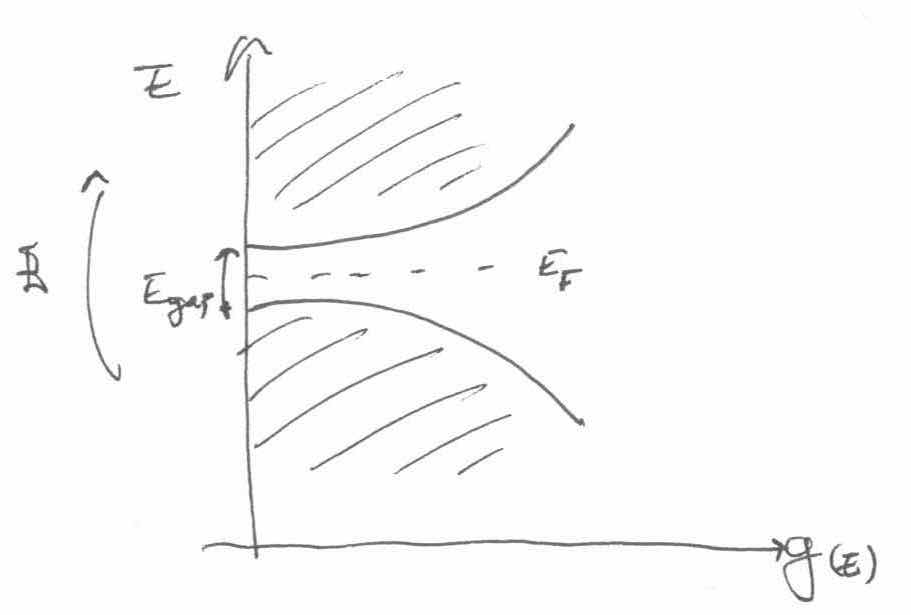
\includegraphics[height=4cm]{images/laser_80_2}
\end{figure}
\noindent
In tempi molto rapidi (pochi fs) gli elettroni eccitati in banda di conduzione e le lacune in banda di valenza termalizzano, cioè si raggiunge una condizione di quasi-equilibrio in cui la probabilità di occupazione degli elettroni in banda di conduzione e valenza è descritta da due distribuzioni di Fermi-Dirac:
\begin{equation*}
f_c(E) = \frac{1}{1+e^\frac{(E - E_{F_c})}{k_B T}}
\end{equation*}
\begin{equation*}
f_v(E) = \frac{1}{1+e^\frac{(E - E_{F_v})}{k_B T}}
\end{equation*}
dove $E_{F_c}$ ed $E_{F_v}$ sono detti quasi-livelli di Fermi in banda di conduzione e valenza. Sia $N$ la densità di portatori iniettati col pompaggio da banda di valenza a banda di conduzione. All'equilibrio termodinamico, se $N=0$, $E_{F_c} = E_{F_v} \equiv E_F$ energia di Fermi.
Se c'è pompaggio, $N\neq 0$, in situazione di quasi-equilibrio $E_{F_c} > E_{F_v}$. Significato fisico di $E_{F_c}$ ed $E_{F_v}$ (a $T\rightarrow0^+$):
\begin{figure}[H]
\centering
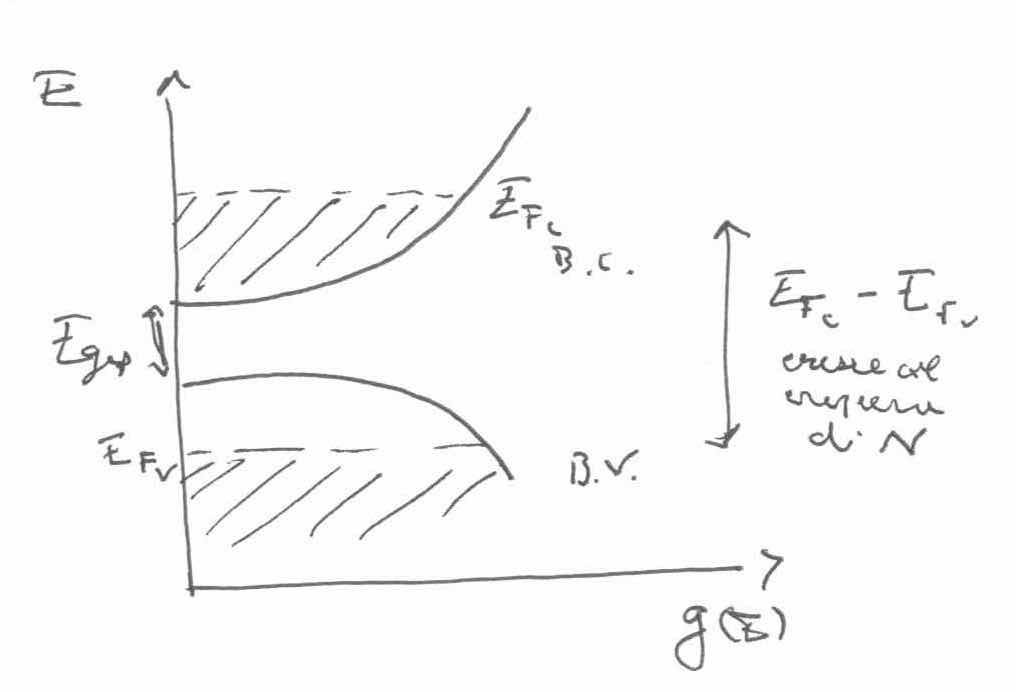
\includegraphics[height=4cm]{images/laser_80_3}
\end{figure}
\noindent
In tempi più lunghi, dell'ordine del tempo di ricombinazione elettrone-lacuna (decadimento radiativo o non radiativo), $\tau \sim 1ns$ nel GaAS, si raggiunge l'equilibrio termodinamico con un solo livello di Fermi $E_F$.

\section{Assorbimento ed emissione stimolata in un semiconduttore. Condizione di Bernard-Duraffourg}
Siano $\psi_v(\*r) = u_{\*k_v} |\*r| e^{i\*k_v \*r}$ e $\psi_c(\*r) = u_{\*k_c} |\*r| e^{i\*k_c \*r}$ che  funzioni di Bloch del cristallo corrispondente alle energie $E_2$, in banda di conduzione, ed $E_1$ in banda di valenza.
\begin{figure}[H]
\centering
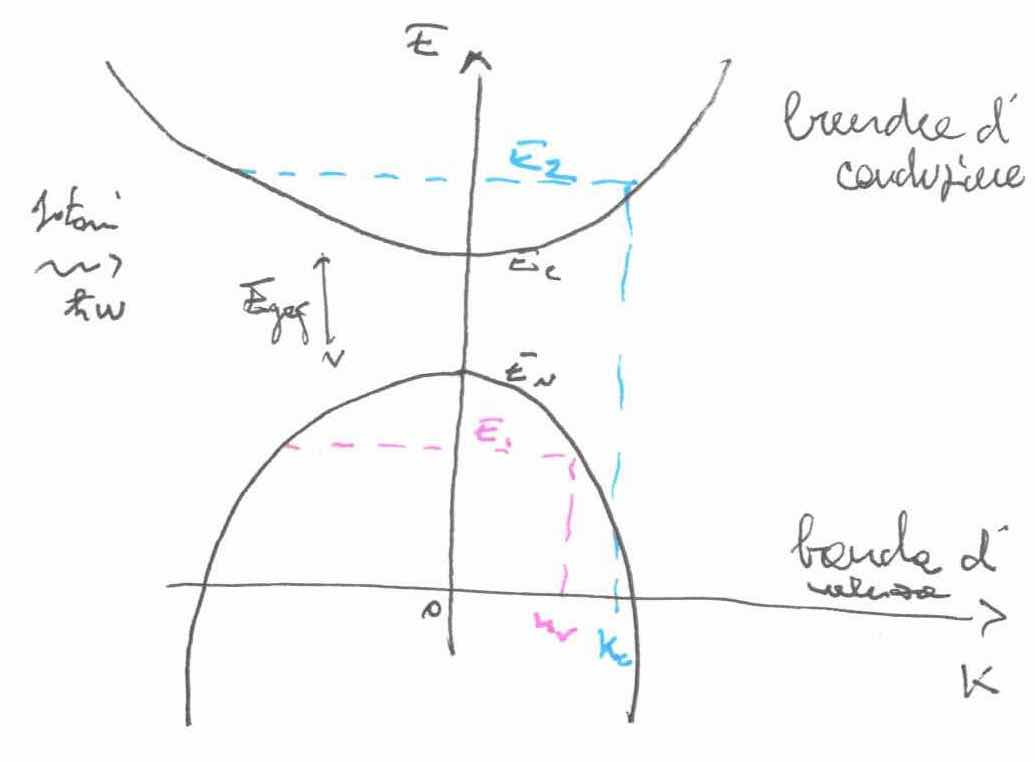
\includegraphics[height=4cm]{images/laser_80_4}
\end{figure}
\noindent
Sul cristallo incide un'onda e.m. monocromatica di frequenza $\w$ e campo elettrico:
\begin{equation*}
\*E(\*r,t) = \*E_0 e^{i\*k_{opt} \*r - i\w t}
\end{equation*}
Applicando la teoria di perturbazione ed assumendo una interazione di dipolo elettrico:
\begin{equation*}
\wh{H}_p = -\*\mu \*E = e\*r \*E
\end{equation*}
è noto che la probabilità nell'unità di tempo di indurre una transizione tra i due stati di Bloch $\psi_c$ e $\psi_v$ vale:
\begin{equation*}
W_{12} = W_{21} = \frac{\pi |\*P_{12}|^2}{2\hbar^2} \delta(\w - \w_0)
\end{equation*}
dove $\w_0 = \frac{E_2 - E_1}{\hbar}$ e $\left|\*P_{12}\right|^2 = \left| \int \psi_c*(\*r) e \*r \*E_0 e^{i\*k_{opt} \*r} \psi_v(\*r) d\*r \right|^2$
Si può dimostrare che $|\*P_{12}|^2 \neq 0$ se è soddisfatta la condizione:
\begin{equation*}
\hbar\*k_c = \hbar \hbar \*k_v + \hbar \*k_{opt}
\end{equation*}
che esprime la condizione di conservazione del momento.
Mentre la $\delta(\w - \w_0)$, cioè $W\neq 0$ se $\w = \w_0$, esprime la conservazione dell'energia. Siccome $|\*k_c|$, $\*k_v|$ sono, come ordine di grandezza, $\frac{\pi}{a}$ (a passo reticolare: tipicamente $a \lesssim 1nm$) mentre $|\*k_{opt}| = \frac{2\pi}{\l}$. Nel visibile ($\l \sim 500 nm$) $|\*k_{opt}| << |\*k_{v,c}|$.
Ciò comporta $\*k_c \sim \*k_v$ (trasmissione verticale nello spazio $\*k$).
Come corollario, segue che non posso usare semiconduttore a gap indiretta (es. Si o Ge) per fare amplificazione stimolata, e quindi un laser. Problema di integrazione tra laser e elettronica.
\begin{figure}[H]
\centering
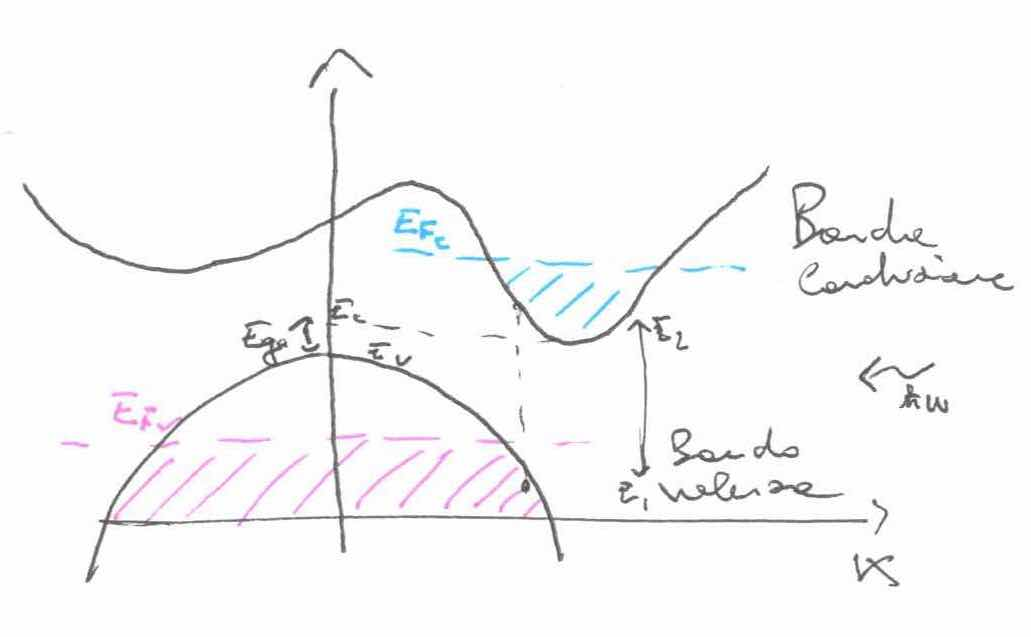
\includegraphics[height=4cm]{images/laser_80_5}
\end{figure}
\noindent
Se si deve avere transizione verticale per conservare il momento, in figura, non si può fare perché l'elettrone che decade dovrebbe andare dove ci sono già presenti due elettroni con spin opposto, quindi violando Pauli.\\
\\
Considero quindi un semiconduttore a gap diretta (es. GaAs, InP) e e chiediamo qual è la condizione tra $E_{F_c}$ ed $E_{F_v}$ per avere amplificazione di luce.
\begin{figure}[H]
\centering
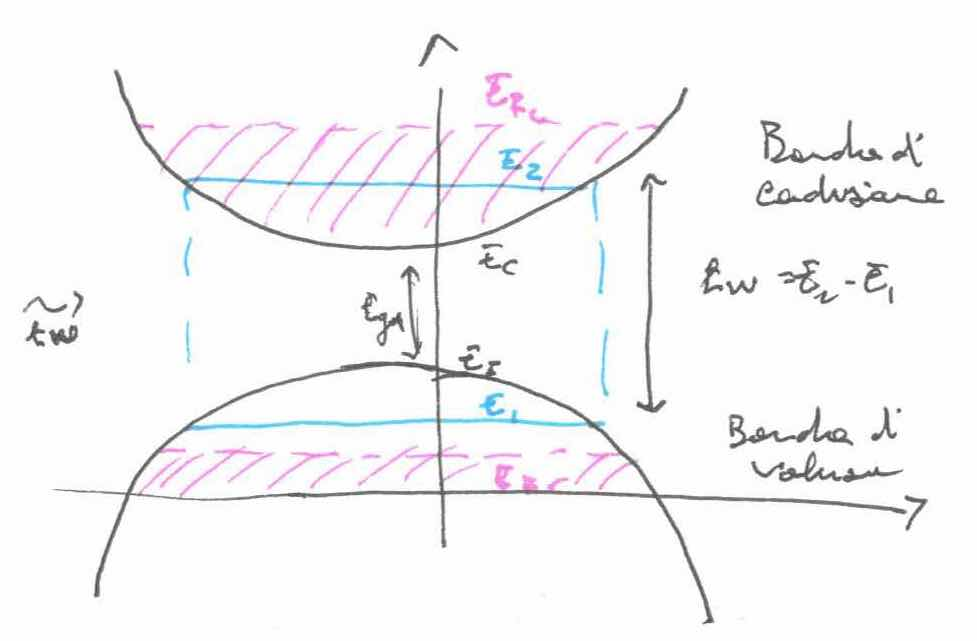
\includegraphics[height=4cm]{images/laser_80_6}
\end{figure}
\noindent
Notiamo che la probabilità che avvenga un processo si assorbimento è proporzionale al termine:
\begin{equation*}
\underbrace{f_v(E_1)}_\text{probabilità di avere elettroni in $E=E_1$} \cdot \underbrace{[1 - f_c(E_2)]}_\text{probabilità di non avere elettroni nel livello $E=E_1$}
\end{equation*}
Similmente, la probabilità che avvenga un processo di emissione stimolata è proporzionale a:
\begin{equation*}
\underbrace{f_c(E_2)}_\text{probabilità di avere elettroni in $E=E_2$ è occupato} \cdot \underbrace{[1 - f_v(E_1)]}_\text{probabilità di non avere elettroni nel livello $E=E_2$ è vuoto}
\end{equation*}
Affinché il semiconduttore amplifichi luce, deve aversi:
\begin{equation*}
f_c(E_2) \cdot [1 - f_v(E_1)] > f_v(E_1) \cdot [1 - f_c(E_2)]
\end{equation*}
cioè:
\begin{equation*}
f_c(E_2) > f_v(E_1)
\end{equation*}
\begin{equation*}
\frac{1}{1 + e^\frac{(E_2 - E_{F_c}}{k_BT}} > \frac{1}{1 + e^\frac{(E_1 - E_{F_v}}{k_BT}}
\end{equation*}
\begin{equation*}
E_2 - E_{F_c} < E_1 - E_{F_v}
\end{equation*}
cioè:
\begin{equation*}
E_2 - E_1 < E_{F_c} - E_{F_v}
\end{equation*}
Del resto, ovviamente $E_2 - E_1 > E_{gap}$ dove:
\begin{equation*}
E_g < E_2 - E_1 < E_{F_c} - E_{F_v}
\end{equation*}
condizione di amplificazione di Bernard-Duraffourg\\
Ciò significa che l'intervallo di frequenze $\w$ che vengono amplificate (banda di guadagno) in un semiconduttore pompato è:
\begin{equation*}
\frac{E_{gap}}{\hbar} < \w < \frac{E_{F_c} - E_{F_v}}{\hbar}
\end{equation*}
Interpretazione ovvia della condizione di Bernard-Douraffourg alla $T=0^+$:
\begin{figure}[H]
\centering
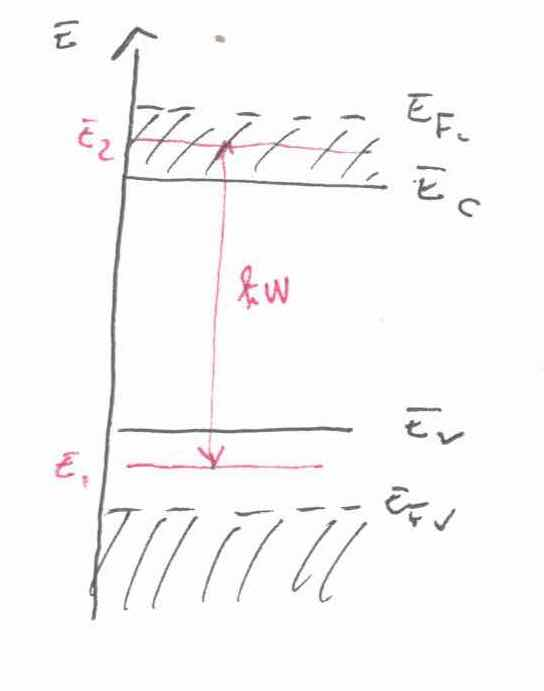
\includegraphics[height=4cm]{images/laser_80_7}
\end{figure}
\noindent
Si noti che per avere amplificazione, $N$ deve essere
\begin{equation*}
N \geq N_{th}
\end{equation*}
dove $N_{th}$ (densità di portatori iniettati a trasparenza) è il valore di $N$ per cui $E_{F_c} - E{F_v} = E_{gap}$.\\
\\
Tipico grafico del coefficiente di guadagno di un semiconduttore:
\begin{figure}[H]
\centering
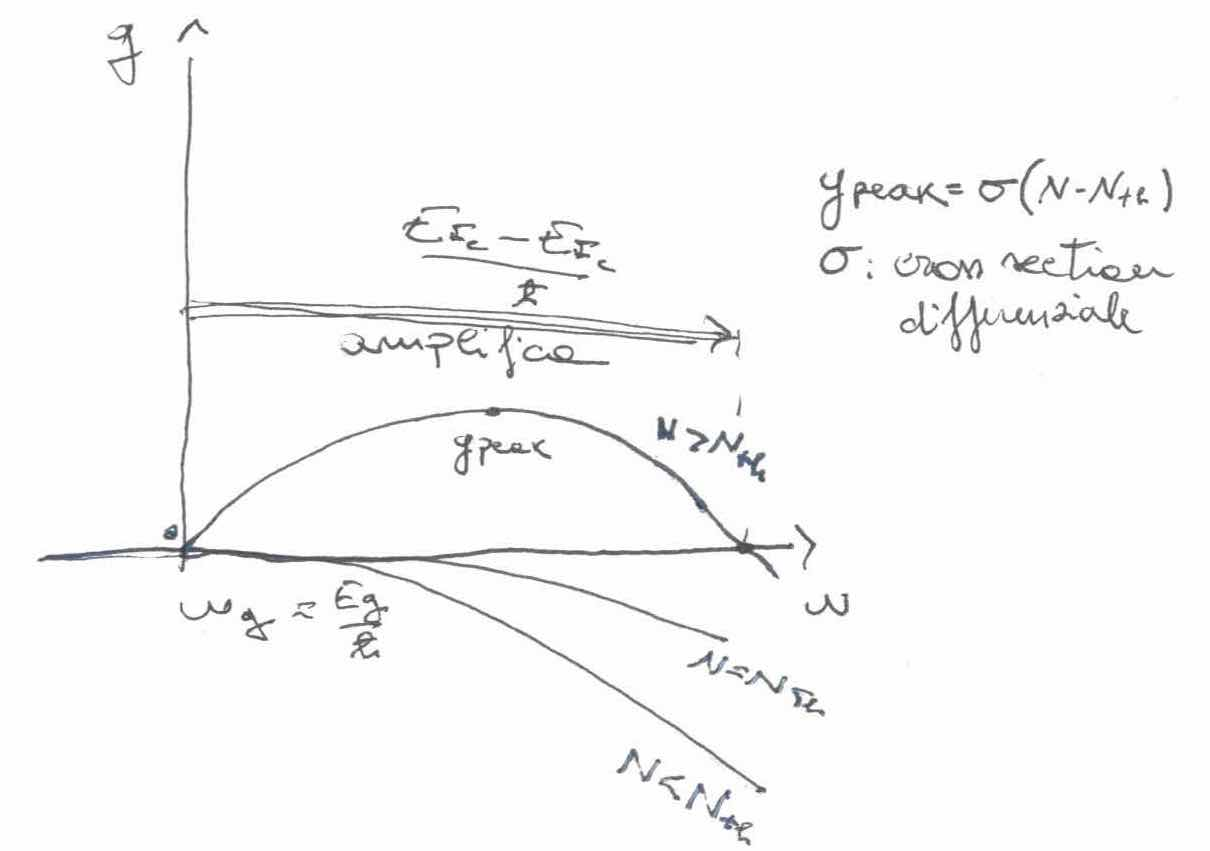
\includegraphics[height=4cm]{images/laser_80_8}
\end{figure}